\documentclass[../class_mech_main.tex]{subfiles}



\DeclareMathOperator{\fpeps}{\frac{1}{4 \pi \epsilon_0}}
\DeclareMathOperator{\fpmu}{\frac{\mu_0}{4 \pi}}


\begin{document}

\chapter{Electrodynamics}

\todo{wouldn't it make sense to have this as chapter 3? Or even 2 (because we often study electrical stuff in analytical mechanics)?}



In classical mechanics, particles are mostly assumed to be really simple. They have a mass and move in some way. But some interactions that are observed experimentally cannot be explained by mass. A natural conclusion is that many real particles (and objects) must have additional properties that explain the observations. Ignoring quantum-mechanical effects for now, perhaps the most important of these properties is \Def{charge}, which induces electromagnetic interactions between charged objects.

From Newtonian theory, we expect that the examination should be relatively simple: through experiments, we find an expression for the electromagnetic force, and then examine all phenomena based on that. As \cite{Griffiths_2017} describes in his introduction to Chapter 1, this can be done, but the resulting expression turns out to be extremely complicated. Therefore, it makes sense to instead build up an understanding using a less ad-hoc approach and study the different regimes first, before combining them all in the most general discussion.


One further note concerns the physical realm of electrodynamics. By examining phenomena exhibited by charges, we wander on the verge between classical, Newtonian physics and relativity. We treat as part of classical physics (the scope of this summary) here because it is not necessary to worry about relativistic effects for many applications (though we could \emph{choose} to do so, as we shall see). But the fact that Einstein developed relativity largely to explain electrodynamics properly should tells us that it is an inherent relativistic theory.


As a last comment, this chapter makes heavy use of math discussed in Sec.~\ref{sec:diff_geo}, where the relation of differential and integral laws is explored.



    \section{Electrostatics}
All charges at rest

        \subsection{The Basics}
We will commonly denote charge by $q$. Every charge is a multiple of an \Def{elementary charge} $e$,
\begin{equation}
    \eqbox{
        q = N e
    }, \; N \in \mathbb{N}
    , \quad
    \eqbox{
        e = 1.602 \cdot 10^{-19} \, \unit{\coulomb}
    } \, .
\end{equation}
This is a crucial difference to masses, where no such \enquote{elementary mass} is known.

A (idealized) concept that is frequently used is that of a point/test charge (closely related to point/test mass), which has all of its charge $q$ concentrated in a point of infinitesimal spatial extent. For a collection of point charges $q_i$, we can use that charge is additive (like mass) to obtain the total charge as
\begin{equation}
    \eqbox{
        Q = \sum_i q_i
    } \, .
\end{equation}
Note that test charges are free to move because the force they exert is proportional to their charge and thus practically zero.

While point charges are a powerful concept, and quite flexible too (in the sense that anything looks like a point charge, if viewed from large enough distance), we cannot always avoid looking in detail at how charges are distributed across a spatial region. In the most general case, we can study this using a charge distribution $\rho = \rho(\vec{r}, t)$, representing charge per volume. (While lines and surfaces are strictly speaking also volumes, just in dimensions lower than three, it is common to use $\lambda, \sigma$ for the density on a line, surface, respectively.) The total charge enclosed in a certain volume $\mathcal{V}$ can then be calculated as
\begin{equation}
    \eqbox{
        Q = \int_\mathcal{V} dq = \int_\mathcal{V} \rho \, d\mathcal{V}
    } \, .
\end{equation}
For a point charge with charge $q$ at $\vec{r}_0$, we can write down the distribution
\begin{equation}
    \eqbox{
        \rho(\vec{r}) = q \, \delta(\vec{r} - \vec{r}_0)
    }
\end{equation}
and similarly, for a collection of charges $q_i$,
\begin{equation}
    \eqbox{
        \rho(\vec{r}) = \sum_i q_i \, \delta(\vec{r} - \vec{r}_i)
    } \, .
\end{equation}
Here we port discrete to continuous by adding a $\delta$-function for each charge, which turns integral into sum.\\


-> note that point charge is flexible notion; if distance to $\vec{r}$ is large, then even macroscopic source can be taken as point charge! (another similarity to mass and gravitation)



Although one can make the point that any electric interaction means we leave the realm of Newtonian physics and enter the one relativity, we still study interactions in terms of forces. The electrical \Def{Coulomb force} (also: \Def{Coulomb's law}) from charge 1 onto charge 2 is
\begin{equation}
    \eqbox{
        \vec{F}_C = \vec{F}_{C, 1 \rightarrow 2}
        = \fpeps q_1 q_2 \, \frac{\vec{r}_{12}}{\norm{\vec{r}_{12}}^3}
        = \fpeps q_1 q_2 \, \frac{\vec{r}_2 - \vec{r}_1}{\norm{\vec{r}_2 - \vec{r}_1}^3}
    } \, .
\end{equation}
where $\vec{r}_{12} = \vec{r}_2 - \vec{r}_1$ is the displacement vector connecting object 1 to object 2 (because of this, it naturally obeys the third law). Similarly to Newton's law of gravitation, it has been found empirically. It, too, obeys the superposition principle,\footnote{As \cite{Griffiths_2017} notes in the first footnote of Chapter 2, this is only the case because $\vec{F}_C$ is linear in the charge. This is truly an empirical insight and should be appreciated appropriately.} which means the Coulomb force from a charge distribution $\rho$ onto a test charge with charge $q$ at position $\vec{r}$ is
\begin{equation}
    \eqbox{
        \vec{F}_C(\vec{r}) = \fpeps q \int_{\mathcal{V}'} \rho(\vec{r}') \frac{\vec{r} - \vec{r}'}{\norm{\vec{r} - \vec{r}'}^3} \, d\mathcal{V}'
    } \, .
\end{equation}
$\epsilon_0$ is a constant, the \Def{permittivity of free space} (\cite{Griffiths_2017} does not like this name, but it is what it is) and in SI units, it takes the value
\begin{equation}
    \eqbox{
        \epsilon = 8.854 \cdot 10^{-12} \unit{\coulomb\squared\per\newton\per\meter\squared}
    }
\end{equation}
which means that the factor $\fpeps$ takes a really large value $\sim 10^{12}$ (which may, of course, be cancelled by small charges or large distances to make the total force small).

Another interesting property of charges that we did not have before with masses etc.~is the following: charges can be positive \emph{and negative}. Thus the Coulomb force can be attractive ($q_1 / q_2 < 0 \Rightarrow \vec{F}_{12} \parallel \vec{r}$) and repulsive ($q_1 / q_2 > 0$), one of many effects that this has.


-> interesting observation: let's say we put two test charges together; of course, they would also have some mass usually, so gravitational interaction would also be present -> thing is: $e \sim 10^{-19}$, while $m_e \sim 10^{-31}$ and the constants in front of charge are also much smaller for gravitational interaction! $G \sim 10^{-11}, 1/\epsilon_0 \sim 10^{12}$; means that on short ranges, electromagnetic interaction is by far dominant; only over long ranges, gravitational takes over because there is no negative mass (for Coulomb force, as we integrate over larger region of space, positive and negative forces will almost completely cancel; mass, on the other hand, only accumulates)


-> nice by Griffiths: Coulomb + superposition principle are all we need for electrostatics; to infer laws, we just exploit mathematical consequences of the specific form it has


-> note that the fact that we can write $\rho(\vec{r}) = \sum_i q_i \, \delta(\vec{r} - \vec{r}_i)$ is consequence of superposition principle; because we can take viewpoint that Coulomb only specifies interaction between two individual particles, and that the total force can be written in such a form inherently relies on us being able to add together forces from each charge thanks to the superposition principle



        \subsection{Electric Field}
Coulomb's law is great for determining the mutual forces of charged bodies onto each other. But sometimes we would like to get such a statement about how a body interacts electrically that is independent of the nature of the second body. This is a very tricky question because a second body is required for an effect/interaction to be measurable at all. Thus we have to apply a trick, which consists of introducing test charge with $q_2 \rightarrow 0$ (similar to the concept of a test mass in mechanics that had $m \rightarrow 0$). The force exerted by this object likewise goes to zero -- but by the third law, so does the force felt by it, which means this is not the measure we seek for the strength. Instead, recognize that, while the force tends to zero, the quotient of force and charge does not. This defines the notion of \Def{electric field} emitted by charge $q$ at position $\vec{r}_0$
\begin{equation}
    \eqbox{
        \vec{E}(\vec{r})
        % = \lim_{q_2 \rightarrow 0} \frac{\vec{F}_C}{q_2}
        = \lim_{q_2 \rightarrow 0} \frac{\vec{F}_{C, \vec{r}_0 \rightarrow \vec{r}}}{q_2}
    } \, ,
\end{equation}
which is our desired measure of how strongly $q$ interacts with its surroundings. (\cite{Griffiths_2017} describes the field as \enquote{force per unit charge}, which is mathematically equivalent to our definition.)


For a collection of charges, described by its distribution, we can always use Coulomb's law to express it more explicitly as
\begin{equation}\label{eq:efield_general}
    \eqbox{
        \vec{E}(\vec{r}) = \fpeps \int_{\mathcal{V}'} \rho(\vec{r}') \frac{\vec{r} - \vec{r}'}{\norm{\vec{r} - \vec{r}'}^3} \, d\mathcal{V}'
    } \, .
\end{equation}
(Important note: careful when carrying out such an integral in practice. Depending on the basis used to write out $\vec{r}, \vec{r}'$, we might have to keep the unit vectors $\unitvec{k}$ in the integrals. For Cartesian coordinates, this is not required, but for curvilinear we cannot avoid this. \cite{Griffiths_2017} therefore advises to always use Cartesian coordinates to calculate electric fields.) In case of a point charge, this yields
\begin{equation}
    \eqbox{
        \vec{E}(\vec{r}) = \fpeps q \frac{\vec{r} - \vec{r}_0}{\norm{\vec{r} - \vec{r}_0}^3}
    } \, .
\end{equation}
-> this particular expression is supremely useful because it is easily integrated in spherical coordinates; using the superposition principle can then, possible, allow us to calculate arbitrary fields more easily (also true if $\rho$ is a function of $r$ only, not direction, or even entirely uniform; then we do not even need to use superposition for this to be true)

-> fields are cool because no matter how charge emitting field is constituted, as soon as we have field, we also get the force on charge $q$ as $\vec{F} = q \vec{E}$ (consequence of superposition principle)


-> but what \emph{is} an electric field truly? This is not so easy to answer, in the end a matter of personal preference of how you think about it. Is certainly a mathematical function that assigns scalar value to each point in space, which measures strength of electric interaction at this point with charge at some fixed position



interesting feature of Coulomb force coming from a charge distribution $\rho$: from entirely mathematical considerations (cf.~Eq.~\eqref{eq:gradient_rnorm}), we can show that it has a \Def{potential} $\varphi$\footnote{Unfortunately, \cite{Griffiths_2017} uses the variable $V$ for our $\varphi$. We do adopt this because $V$ is used for the potential of the Coulomb force below, continuing how things are named in Newtonian physics.} (though this also makes sense physically, Coulomb is a central force, and those always have a potential); this is quantified equivalently by
\begin{equation}
    \eqbox{
        \vec{E} = - \grad \varphi
    }
    \quad \quad
    \eqbox{
        \varphi(\vec{r}_0) - \varphi(\vec{P}) = - \int_{\vec{P}}^{\vec{r}_0} \vec{E}(\vec{r}) \cdot d\vec{r}
    } \, .
\end{equation}
(One quick note: the lower limit $\vec{P}$ just comes out as an integration constant that vanishes when taking a gradient, so it is arbitrary. This is a common theme with potentials, only potential differences are uniquely determined. It is common to choose $\vec{P} = \infty$ because for real-world electric fields, $V(\infty) = 0$. If you have a textbook problem where this is not the case, you are free to choose $\vec{P}$ differently.) The explicit path $\vec{C}$ taken between the integration limits does not influence the result here (a consequence of the fundamental theorem of calculus, due to the existence of the anti-derivative $V$; equivalently, a consequence of $\curl \vec{E} = 0$), so we straight up omitted here and just wrote down the integration limits.


Let us now collect a few notes regarding the potential, especially regarding names in this context:
\begin{itemize}
    \item Careful with the name \enquote{potential}. In mechanics, potentials of forces were directly equal to energy. However, \enquote{potential} is a more general, in fact mathematical term, and we are looking at the potential of a field in case of $\varphi$. It is possible to define an analogous potential for the Coulomb force in
    \begin{equation}
        \eqbox{
            V \coloneqq q \varphi
        } \, ,
    \end{equation}
    and as we will see in Sec.~\ref{subsec:estatics_energy}, this potential is indeed related to the energy of an electrostatic field. But the initial point stands, we have to be more careful with the identification because several notions of potential exist.
    
    (Note that the existence of $V$ implies that the Coulomb force is conservative. We could have seen this immediately since it is a central force.)
    
    
    \item A potential difference $\Delta \varphi$ between two points is called \Def{voltage}. This name is closely connected to the unit of the potential, which is defined as \Def{volt}. Since the expression of $\varphi$ is just force ($\unit{\newton}$) multiplied with $\unit{\meter}$ (due to different power in norm) and divided by $\unit{\coulomb}$ (because we are missing a $q$); thus,
    \begin{equation}
        \eqbox{
            \qty[\varphi] = \unit{\newton \meter \per \coulomb} \unit{\joule \per \coulomb} \eqqcolon \unit{\volt}
        }
    \end{equation}
    (I guess here it would be cool to use $V$ instead of $\varphi$...)


    \item The remarkable fact that all information from a \emph{vector} field (three components/numbers for each point in space) is already contained in a \emph{scalar} field (one number for each point in space) is quickly explained by the fact that the specific form and physical origin $\vec{E}$ do not permit fully independent components (e.g., the curl vanishing is inherently a condition on combinations of components, essentially reducing the degrees of freedom of them)
\end{itemize}


Coulomb force has superposition principle, electric field has it, and due to the linearity of the gradient, the potential also has it. Similarly, the preceding discussions allow us to write down a general expression for $\varphi$. Eq.~\eqref{eq:efield_general} implies
\begin{equation}\label{eq:potential_general}
    \eqbox{
        \varphi(\vec{r}) = \fpeps \int_{\mathcal{V}'} \rho(\vec{r}') \frac{1}{\norm{\vec{r} - \vec{r}'}} \, d\mathcal{V}'
    } \, .
\end{equation}
(Note that the sign in $\norm{\vec{r} - \vec{r}'}$ is important here because it determines the sign in the electric field Eq.~\eqref{eq:efield_general}.)


-> existence of potential implies curve-integrals are path-independent; we define \Def{voltage} based on this, as difference of scalar potentials; is related to work in straightforward manner, via $W = q U$ (is amount of work done on a charge, independent of actual charge that is moved, right? Same relation as between electric field and force) \todo{rather introduce notion of voltage later on?}


-> say we have sphere of radius $R$ with uniform surface charge. What is potential? Gauss's law yields field outside of sphere (the cool trick with symmetry), while inside is zero (because no charge enclosed). So for $r \geq R$, we can obtain $\varphi$ by the usual integration of $E$ from our reference point $\infty$ to $r$. What about $r < R$? Field vanishes inside, does it too? Well, no, since we start our integration from $\infty$ and not zero. But intuition is not completely off, $\rho(\vec{r}) = 0$ for these points, so $\varphi(r > R) = \varphi(R) = \mathrm{const}$ (as it should, field as gradient of potential must vanish)

-> now say we have charge enclosed in sphere of radius $R$



            \paragraph{Field Lines}
convenient tool to visualize vector fields, replace drawing the actual vector with its magnitude in many points in space

-> magnitude of field can now be read off from density of field lines


some rules:

field lines are drawn from positive to negative charges, i.e.~they represent direction of force acting on a particle with positive charge; to make things even more clear, they begin on negative charges and end on positive ones (so electrons move against the field lines in an electric field)

if we start to draw a field line, we must either also draw its ending (though we might leave out some part in between, in case they extend too far out) or they must go to infinity; this must be the case since $\vec{E}$ is divergence-free in free space

be consistent: if charge $q$ has four field lines, then a charge $2q$ in the same plot should get eight lines (this is motivated by Gauss's law, which we learn about in a minute)


another possibility to visualize fields: \Def{equipotential lines}, i.e.~lines where $V = \mathrm{const}$; these are everywhere perpendicular to the field lines



        \subsection{Maxwell Equations}

straightforward question: what is \enquote{total electric field} of some charge distribution $\rho$? For that, integrate over surface $\mathcal{S}(\mathcal{V})$ enclosing volume $\mathcal{V}$ in which $\rho$ is located spatially. We can do that:
\begin{equation}\label{eq:gauss_law_integral}
    \eqbox{
        \oint_{\mathcal{S}(\mathcal{V})} \vec{E} \cdot d\vec{\mathcal{S}} = \frac{Q}{\epsilon_0}
    }
\end{equation}
where $d\mathcal{S}$ is surface element of $\mathcal{S}$, which is formally turned into a vector by multiplying it with the normal vector $\vec{n}_\mathcal{S}$ of the surface.\footnote{The job of the normal vector is to extract the component of $\vec{E}$ that actually flows through the surface (any flux tangential to the surface is not interesting for the intended use of calculating flux through $\mathcal{S}$).} In words: flux of electric field through a surface is proportional to charges inside! In particular, no charges in $\mathcal{V}$ means that net flow of $\vec{E}$ through $\mathcal{S}$ is zero -- independent of its exact shape, just has to be connected, closed


-> this is first Maxwell equation (or rather integral version thereof)

-> very interesting note: any $1/r^2$ force has its own Gauss law because the only thing we rely on is surface $\propto r^2$, which then cancels radius from force (why is this true for surface? Well, we can always choose \enquote{equivalent} surface to integrate over, where all charges are enclosed as well, namely a sphere of a certain radius -> I think this is the reasoning, not 100\% sure)

moreover, Gauss's law (the other one, relating surface integral to volume integral over divergence) can be used to obtain
\begin{equation*}
    \frac{Q}{\epsilon_0} = \frac{1}{\epsilon_0}\int_\mathcal{V} \rho(\vec{r}) \, d\mathcal{V} = \oint_{\mathcal{S}(\mathcal{V})} \vec{E} \cdot d\vec{\mathcal{S}} = \int_\mathcal{V} \div \vec{E} \, d\mathcal{V}
\end{equation*}
which yields the differential version of first Maxwell,
\begin{equation}\label{eq:gauss_law_differential}
    \eqbox{
        \div \vec{E} = \frac{\rho}{\epsilon_0}
    }
\end{equation}
(Notice how this implies $\vec{E}(\vec{r}) = \fpeps \frac{\div \vec{E}(\vec{r}')}{\norm{\vec{r} - \vec{r}'}} \, d\mathcal{V}'$, which is a reflection and consequence of the Helmholtz theorem \ref{thm:helmholtz_thm})


-> differential might be more concise, but integral one is immensely powerful: it yields total charge in a volume, we only have to measure electric field on some closed surface around it; or, if we know (i) the total charge in the volume and (ii) that the electric field is uniform, it is a shortcut to $\vec{E}$, by using the \Def{Gaussian surface} technique: if the volume $\mathcal{V}$ is sufficiently symmetric (\cite{Griffiths_2017} quotes three possibilities that work: sphere, cylinder, plane; basically shapes for which we have nice curvilinear coordinates tailored to them, so that $\vec{E} \parallel \vec{S}_n$) and the charge density indeed uniform, we can indeed place a volume $\mathcal{V}'$ of the same shape (sphere around sphere, etc) around $\mathcal{V}$, but so that $\mathcal{V}'$ is larger than $\mathcal{V}$; we might still apply it if this symmetry is not present though, namely for systems where individual parts have such a symmetry (compute individual fields, use superposition)


second Maxwell equations is more straightforward:
\begin{equation}\label{eq:maxwell_estat_two}
    \eqbox{
        \curl \vec{E} = 0
    }
    \quad \Leftrightarrow \quad
    \eqbox{
        \oint_\mathcal{C} \vec{E} \cdot d\vec{r} = 0
    }
\end{equation}
where $\mathcal{C}$ is a closed curve (as indicated by use of $\oint$ instead of $\int$)

-> proof is relatively simple: calculate line integral along closed loop of field generated by point charge (turns out to be zero), apply Stokes's theorem to conclude vanishing curl for this setup, use superposition principle to conclude this must be true for general charge distribution (works because curl is linear)



        \subsection{Poisson Equation}
In terms of the potential, Maxwell's equations imply that the potential fulfills the \Def{Poisson equation}
\begin{equation}\label{eq:poisson_eq}
    \eqbox{
        \nabla^2 \varphi = - \frac{\rho}{\epsilon_0}
    } \, .
\end{equation}
Yes, it is actually a consequence of \emph{both} Maxwell equations. While this particular form is derived by inserting $\vec{E} = - \grad \varphi$ into the first Maxwell equation, the second one is implicitly used in the fact that we work with a potential, the existence of which is only asserted by the second Maxwell equation.

-> interesting: we cannot write down analytical, general solutions to PDEs; is because is not possible to write things out with finite number of constants


For the positions where no charges are present, Poisson's equation turns into the \Def{Laplace equation}
\begin{equation}\label{eq:laplace_equ}
    \eqbox{
        \nabla^2 \varphi = 0
    } \, .
\end{equation}
Discussing and solving this equation not only solves physical problems in many cases (namely when no charge is located in the volume where we wish to obtain $\varphi$), but also because an inhomogeneous differential equation like the Laplace equation is always solved by a linear combination of a solution to the full, inhomogeneous equation plus a solution to the corresponding homogenous equation (one can always add the latter and the inhomogeneous equation is still fulfilled). In short, we can learn a lot about the solutions of Poisson's equation by studying those to Laplace's.

-> interesting features are (i) each value of solution is average of its neighboring values and (ii) extrema of $V$ must occur at the boundaries of the volume we integrate over, Laplace's equation does not permit local minima/maxima (\cite{Griffiths_2017} says the following about this: \enquote{Laplace's equation picks most featureless function possible, consistent with the boundary conditions} and \enquote{a harmonic function in two dimensions minimizes the surface area spanning the given boundary line}, where harmonic functions are a general name for the solution of Laplace's equation)

-> \emph{very} interesting: the value of $\varphi$ at point $\vec{r}$ is equal to the average value of $V$ over a spherical surface of radius $R$ centered at $\vec{R}$,
\begin{equation}
    V(\vec{r}) = \frac{1}{4\pi R^2} \oint_\mathrm{sphere} V \, d\mathcal{S}
\end{equation}
(for solution of Laplace's equation)



        \paragraph{Why Use It?}
We have started to look at some of the features and difficulties of dealing with the Poisson equation. But we have not justified why it should even be used. Why should we even want to use this partial differential equation of second order? After all, just give me the charge distribution $\rho$ and I can calculate $\varphi$ and $\vec{E}$ using the formulas \eqref{eq:efield_general}, \eqref{eq:potential_general}.

However, these equations are all stated in terms of integrals that are not particularly easy to evaluate. (Well, at least analytically, since it is seldomly the case that geometries of bodies are sufficiently simple to allow us to use some of the tricks we have seen before. Integrating numerically is also not trivial, though. Partly, this is because the geometry of the involved bodies might be hard to parametrize. \todo{this must play a role here, right?}) More importantly, however, the integration only works if we indeed know $\rho$. As it turns out, this is by no means guaranteed and for many applications, we only know the total charge of a body, but have no clue about how this charge is distributed (which is quite reasonable, there might be a lot of motion due to the interaction of charges, until the equilibrium is reached).

Hence we are sometimes forced to solve differential equations instead of doing integration. If we are indeed interested in positions where $\rho(\vec{r}) = 0$, then we are left with the Laplace equation or equivalently the homogenous Maxwell equation. (The crucial difference to the the integrals in Eqs.~\eqref{eq:efield_general}, \eqref{eq:potential_general} is that they require $\rho$ even if we just want the field in positions where $\rho = 0$.) Having to choose between the two is then a matter of making the most economic decision: we can choose a partial differential equation of second order for a scalar field or a partial differential equation of first order for three scalar fields (each component enters in the Maxwell equation). This is why solving the Laplace/Poisson equation is an important task in electrostatics.



-> Fig.~2.35 of \cite{Griffiths_2017} is incredible, shows how we may translate between $\rho, \vec{E}, \varphi$



            \paragraph{Boundary Conditions}
Differential equations must always be supplemented with a set of suitable boundary conditions. A priori, it is not clear which boundary conditions are suitable, in fact it can be quite difficult to specify them (must be restrictive enough that they constrain solutions, but not too restrictive that they prohibit us from finding a solution at all). For the Laplace and Poisson equation in particular, there are a several possible choices, which each come with a theorem proving that the choice makes a \enquote{good} boundary condition (in form of a uniqueness theorem, which means that the condition permit finding a unique solution).


\begin{thm}[First Uniqueness Theorem]\label{thm:uniqueness_poisson_1}
    The solution to Laplace's equation in a volume $\mathcal{V}$ is uniquely determined if the potential is specified on the boundary surface $\mathcal{S} = \partial \mathcal{V}$.

    This implies that the potential, a solution to Poisson's equation, in a volume $\mathcal{V}$ is uniquely determined if the charge density throughout all of $\mathcal{V}$ along with the potential value on all boundaries is specified.
\end{thm}
This is a remarkable statement: if I find any solution for a given boundary condition, then it is \emph{the} solution -- there is no other one.
-> there are uniqueness theorems, which guarantee that if we find solution, it is the only one


What if we do not know charge density? Was one of the motivations to treat Poisson at all... Luckily, there is another theorem for this case. (Note that we have not formally introduced conductors yet... That is what happens when you follow a book, but structure your notes differently, I guess, but for us a conductor can just be any surface with uniform charge density on it at the moment.)

\begin{thm}[Second Uniqueness Theorem]\label{thm:uniqueness_poisson_2}
    In a volume $\mathcal{V}$ surrounded by conductors and containing a specified charge density $\rho$, the electric field is uniquely determined if the total charge of each conductor is given.
\end{thm}
Hence, what we need is the charges on all conducting surfaces around (inside and outside) the volume of interest. (The region as a whole can be bounded by another conductor or else unbounded, whence the outer boundary is at infinity.)


-> these have interesting consequences for electrostatics, even when we do treat it by solving Laplace's equation: if we find solution for electric field that fits boundary conditions, then this is the unique solution to the problem; the way in which we obtain the solution does not matter. This justifies, for example, the method we had used before to determine uniform electric fields for symmetric configurations

-> one application for this is discussed in next subsection, where we show how to circumvent cumbersome solution techniques like the separation of variables that are normally used to solve Laplace's equation (and that also do not work all the time)



        % \subsection{Image Charges}
            \paragraph{Image Charges}
Here we present a general method to solve Poisson equation subject to certain boundary conditions. The idea is best explained by means of an explicit example: take the problem where a charge is placed in front of a conductor (of infinite length). 

-> idea: to get, for example, field of one charge that shall be perpendicular to certain surface, we can place image charge(s) at certain spot so that field lines cross surface in desired manner (mimick boundary conditions)

-> important detail: the image charges we place must be outside of the area where we are interested in the field, just outside (where, e.g., ground of the charged plate or something is)

-> why does it work? Because we have proven uniqueness theorems for the solution (in particular the first one, \ref{thm:uniqueness_poisson_1}), which means even if we find it by guessing, it is the correct one! And even if the setup studied is entirely different, as long as boundary conditions are same

-> can be done in general, though it is not always easy (highly dependent on geometry of the setup)

% -> isn't idea also somewhat borrowed from multipole expansion? Which allows us to describe arbitrary distribution with discrete number of particles; basically same is now done for boundary conditions


-> potential is guaranteed to agree between the setups; but this determines e-field and force, so they agree too. From this we can, e.g., compute force from conductor onto the charge (noting that $\eval{\frac{\vec{r} - \vec{r}'}{\norm{\vec{r} - \vec{r}'}}}_{\vec{r}' = 0} = 0$ because it is zero component-wise; is single application of l'Hospital)

-> BUT: energy is not same; should also make sense, since image charges only apply to region \emph{above} the plate, but energy calculated for point charge takes into account all space, not just above; by symmetry argument, energy in field of conductor plate is half of the result



        \subsection{Energy}
        \label{subsec:estatics_energy}
\todo{move in front of Poisson equation section, in case we deal with energy of image charges. Or make image charges a subsection again and move it between energy, multipole expansion}
In this section, we answer a very simple question: what is the energy of an electric field? (By \enquote{simple} we mean conceptually simple, as we do not know how simple it is to answer.)

In Newtonian physics, energy is the ability to do work. We continue in this vein, starting with a simple example. Suppose some electric field $\vec{E}$ is present. Then we can use the definition of work to require how much of it is required to move a single charge $q$ between two positions $\vec{a}, \vec{b}$:
\begin{equation}\label{eq:work_test_part_1}
    W = \int_{\vec{a}}^{\vec{b}} \vec{F} \cdot d\vec{r} = \int_{\vec{a}}^{\vec{b}} q \vec{E}(\vec{r}) d\vec{r} = - q \qty[\varphi(\vec{b}) - \varphi(\vec{a})] = - \qty[V(\vec{b}) - V(\vec{a})]
    \, .
\end{equation}
% This is not a surprising result, it matches what we are used to from Newtonian physics. It represents the work that somebody (or something) has to do in order to move a point charge $q$ through the electric field $\vec{E}$, which can be positive (force between $q$ and the field is repulsive) or negative (force between $q$ and the field is attractive).
This is not a surprising result, it matches what we are used to from Newtonian physics. It represents the amount of resistance by the Coulomb upon moving a point charge $q$ through the electric field $\vec{E}$. Conversely, somebody (or something) has to do the work $- W$ on the charge for it to be able to move through the electric field (we need a minus sign here because the force exerted must always be exactly opposite the Coulomb force). $W$ can be positive (force between $q$ and the field is repulsive) or negative (force between $q$ and the field is attractive).

To make sure we do not \enquote{miss out} on work that needs to be done against the electric field, it is common to choose $\vec{a} = \infty$. The work required to move a charge $q$ to the position $\vec{r}$ (which replaces $\vec{b}$ now) is then simply
\begin{eqnarray}\label{eq:work_test_part_2}
    \eqbox{
        W \coloneqq W_{\infty \rightarrow \vec{r}} = V(\vec{r}) - V(\infty) = V(\vec{r}) = q \varphi(\vec{r})
    }
\end{eqnarray}
where the second equality assumes we have $\infty$ as our reference point for $\varphi, V$, so that $V(\infty) = 0$. The last equality means electric work is charge multiplied by voltage. (A quick sanity check: the voltage $\varphi$ had unit volts, charge has coulomb. But since volt = joule per coulomb, work indeed comes out as joule, so everything is nice and consistent.)


Just like before, this result for a single point charge can be generalized to other charge distributions. We do just that now, calculating how much work is required to assemble a certain collection of charges from $\infty$. For the first particle, there is no electric field to do work against, so $W_{\infty \rightarrow 1} = 0$); for the second particle, one has to do work against $\vec{E}_1$; for the third one, against $\vec{E}_1 + \vec{E}_2$; etc. Using the superposition principle for the scalar potential, we end up with
\begin{equation}\label{eq:work_discr_distr}
    W
    = \sum_i W_{\infty \rightarrow i}
    = \sum_i q_i \sum_{j < i} \varphi_j(\vec{r}_i)
    = \frac{1}{2} \sum_{\underset{i \neq j}{i, j}} q_j \varphi_i(\vec{r}_j)
    = \frac{1}{2} \sum_j q_j \varphi_{\qty{q_i}_{i \neq j}}(\vec{r}_j)
\end{equation}
where the weird subscript of $\varphi$ is used to denote the potential of all charges, except for the $j$-th one. We were able to obtain this result because we replaced the sum over $j < i$ with two sums of this kind (accounting for this the factor $\frac{1}{2}$) because it is easier to evaluate. (Note that this expression, as all before, encapsulate only interaction energy, not self energy.)

\todo{this does not account for energy needed to keep the distribution together, right? So I guess we assume that all particles are brought in instantaneously, immediately one after the other. But then I wonder how this is a good model of true energy density...}

in the continuum limit, this reads
\begin{equation}\label{eq:work_cont_distr_1}
    \eqbox{
        W = \frac{1}{2} \int_{\mathcal{V}} \rho(\vec{r}) \varphi(\vec{r}) d\mathcal{V}
    } \, .
\end{equation}
In contrast to Eq.~\eqref{eq:work_discr_distr}, self-energy is now included because we integrate over \emph{all} of $\varphi$ and not just $\varphi_{\qty{q_i}_{i \neq j}}$. By choosing to integrate not only over $\mathcal{V}$, but over all space, this takes the form
\begin{equation}\label{eq:work_cont_distr_2}
    \eqbox{
        W = \frac{\epsilon_0}{2} \int \norm*{\vec{E}}^2 \, d\mathcal{V} \eqqcolon \int w(\vec{r}) \, d\mathcal{V}
    }
\end{equation}
with the energy density $w$ (of electrostatics).


Discussion: Eq.~\eqref{eq:work_test_part_2} does not contain self-energy, while Eq.~\eqref{eq:work_cont_distr_2} does. Therefore, the former is energy we gain when disassembling the charge configuration, but the latter is not.

-> there is good and bad to both: good for first expression is that we do not create charges in practice, we just use already existing electrons etc., so not including self-energy is the correct thing; good for second expression is that it is more complete as it truly contains the total energy stored in the charge distribution (which is nicer if we actually want energy of it, not work needed to assemble)

-> general issue: energy of point charge is (just use Eq.~\eqref{eq:work_cont_distr_2} with single $\delta$-function for $\rho$) infinite. This is not because formula is at fault, but because the concept is weird. Actually, that makes matters worse, though, because point charges are an integral concept in electrodynamics, so the fact that their energy diverges is concerning.

-> very interesting question: where exactly is the energy we have just calculated stored? In the charges? Or is it spread throughout the volume? Well, right now both interpretations are totally valid. We will see later on, though, that it is more customary to think about it as being stored in the field, as a density $w$ throughout all space (this is the preferred interpretation for radiation theory and also general relativity)

-> just like kinetic energy is not additive although velocities are, the electric energy does not obey superposition principle although force/field/potential do (is quadratic in field after all)



        \subsection{Multipole Expansions}
Multipole expansions are a frequently used tool in electrodynamics. The basic idea is to simplify terms of the kind $\frac{1}{\norm{\vec{r} - \vec{a}}}$ by using the general result
\begin{equation}\label{eq:multipole_exp_general}
    \eqbox{
        \frac{1}{\norm{\vec{r} - \vec{a}}}
        % \simeq \frac{1}{r \norm{\vec{e}_r - \frac{a}{r} \vec{e}_a}}
        \simeq \frac{1}{r} + \frac{\vec{r} \cdot \vec{a}}{r^3} + \frac{3 (\vec{r} \cdot \vec{a})^2 - r^2 a^2}{2 r^5}
    } \, .
\end{equation}
(For the explicit calculation, see Eq.~\eqref{eq:eq:multipole_exp_general_calc}.)


-> for large enough distances, we can replace with first/second order to really good approximation! Especially useful to calculate field generated by some distribution, this way we can avoid the really nasty integrals, e.g., for potentials and fields!


Is useful because it allows analysis of arbitrary potential in far-field limit $\norm{\vec{r}} \gg R$, where $R$ is the radius of a ball we assume that the charge distribution can be enclosed in. If this is warranted, so is the expansion
\begin{align}
    \eqbox{
        \varphi(\vec{r})
    }
    &\simeq \fpeps \int_\mathcal{V} \rho(\vec{a}) \qty[\frac{1}{r} + \frac{\vec{r} \cdot \vec{a}}{r^3} + \frac{3 (\vec{r} \cdot \vec{a})^2 - r^2 a^2}{2 r^5}] d^3a
    \\
    &= 
    \eqbox{
        \fpeps \qty[\frac{Q(\mathcal{V})}{r} + \frac{\vec{r} \cdot \vec{p}}{r^3} + \frac{1}{2} \sum_{i, j} \frac{Q_{ij}}{r^5} \vec{r}_i \vec{r}_j]
    }
\end{align}
where for instance
\begin{equation}
    \eqbox{
        \vec{p} = \int_\mathcal{V} \rho(\vec{a}) \vec{a} \, d^3a
    } \, ,
\end{equation}
which is independent of $\vec{r}$. For the rest of this subsection, our goal is to give a physical meaning to each order of the expansion, and also find expressions for the unknown factors. The general idea will be to find a setup that eliminates terms from all order below the one we wish to investigate. This will allow to investigate each order separately.



            \paragraph{Monopole}
Easiest description: $\mathcal{V}$ is so small that it appears as point with no spatial extent. In that case, it can be treated as point charge with charge $Q(\mathcal{V})$. This is the easiest, most simplified description that one can think of, so it naturally corresponds to leading order term
\begin{equation}
    \eqbox{
        \varphi_\mathrm{mono}(\vec{r}) = \fpeps \frac{Q(\mathcal{V})}{\norm{\vec{r}}}
    } \, .
\end{equation}



\begin{figure}
    \centering

    \subfloat[Positive charge]{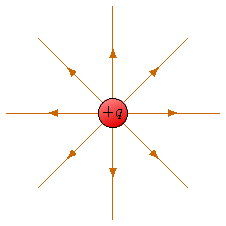
\includegraphics[page=1, width=0.25\textwidth]{pictures/monopole.pdf}}%
    \hspace*{0.1\textwidth}%
    \subfloat[Negative charge]{\includegraphics[page=2, width=0.25\textwidth]{pictures/monopole.pdf}}

    \caption{Monopoles emitted by oppositely charged particles. Taken from \url{https://tikz.net/electric_fieldlines1/}.}
    \label{fig:monopoles}
\end{figure}



            \paragraph{Dipole}
In order to eliminate the monopole term, we need $Q(\mathcal{V}) = 0$. The simplest way to achieve this is to place to point charges with opposite charge together. Placing particle 1 (charge $-q$) in the origin and particle 2 (charge $q$) at a position $\vec{a}$,\footnote{Note that it does not matter whether $q > 0$ or $q < 0$. It is just important that the particles have opposite charge.} the field of this setup is just the superposition
\begin{equation}
    \eqbox{
        \varphi_\mathrm{dipo}(\vec{r})
    }
    = \fpeps \qty[\frac{-q}{\norm{\vec{r}}} + \frac{q}{\norm{\vec{r} - \vec{a}}}]
    \eqbox{
        \simeq \fpeps \frac{\vec{r} \cdot \vec{p}}{x^3}
    }
\end{equation}
where we defined the \Def{dipole moment}
\begin{equation}
    \eqbox{
        \vec{p} \coloneqq q \vec{a}
    } \, .
\end{equation}
Not only does this approximated expression look like the second term in Eq.~\eqref{eq:multipole_exp_general}, it \emph{is} this expression for the physical setup of two oppositely charged point masses:
\begin{equation}
    \eqbox{
        \rho(\vec{r}) = q \delta(\vec{r} - \vec{a}/2) - q \delta(\vec{r} + \vec{a}/2)
    } \, .
\end{equation}
Therefore, the second term does indeed represent 


-> in multipole expansion, we have carried out far-field limit, so to understand connection to different order terms better we should do same now for dipole potential; this is what happens in second equality (along with $\lim_{a \rightarrow 0, q \rightarrow \infty}$ so that product remains well-defined) -> this would be the ideal/pure dipole

-> it is not always clear whether the actual dipole with most general field or the second, approximate formula is meant, but we do our best to distinguish the two (\cite{Griffiths_2017} calls these two physical dipole, referring to the full potential with $Q(\mathcal{V}) = 0$ where highest order is dipole term, and ideal/pure dipole, referring to equations where we actually add positive and negative charge -> ahhh no, that's wrong; for some reason, he calls pure dipole the term that comes out of approximation and physical dipole the one comprised of two charges; I do not like this and will not adopt)

-> means I can do two things to improve approximation: increase $r = \norm{\vec{r}}$ or decrease $a$ (we want/need $r \ll a$)


-> field generated by pure dipole can simply be calculated as
\begin{align}
    \vec{E}(\vec{r}) &= - \grad V(\vec{r}) = - \fpeps \qty[-q \frac{-\vec{r}}{r^3} + q \frac{-(\vec{r} - \vec{a})}{\norm{\vec{r} - \vec{a}}^3}]
    \\
    &\simeq \fpeps q \frac{\vec{a})}{\norm{\vec{r} - \vec{a}}^3} = \fpeps \frac{\vec{p})}{\norm{\vec{r} - \vec{a}}^3}
\end{align}



We have mainly studied the potential and field associated with a dipole until now. But what about its interaction with another electric field $\vec{E}(\vec{r})$? From the most general expression, we quickly arrive at the following force on the dipole:
\begin{equation}
    \eqbox{
        \vec{F}(\vec{r})
    }
    = - q \vec{E}(\vec{r}) + q \vec{E}(\vec{r} + \vec{a})
    \eqbox{
        \simeq \grad \vec{p} \cdot \vec{E}(\vec{r})
    }
    \eqqcolon - \grad V(\vec{r})
    \, .
\end{equation}
First of all, that means the dipole force has a potential, i.e.~is conservative. Moreover, in a spatially homogenous field, there is no force acting on a dipole. Nonetheless, there is an effect of the force, namely a torsion
\begin{equation}
    \eqbox{
        \vec{M}
        = \vec{a} \cross q \vec{E}(\vec{r} + \vec{a})
        = \vec{p} \cross \vec{E}(\vec{r})
    }
\end{equation}
acting on a dipole, which leads to change in orientation until $\vec{p} \parallel \vec{E}$ where the potential is minimized\footnote{While an antiparallel configuration formally also extremizes the potential, this configuration corresponds to a maximum, which means it is not stable.} This can be understood similar to a statement in terms of center of mass: the dipole itself is not moving in the electric field, but it constituents do; via the complex interplay of both forces moving in the external $\vec{E}$-field while the two particles still interact, the total effect is merely a rotation of the dipole.



\begin{figure}
    \centering

    \subfloat[Near field]{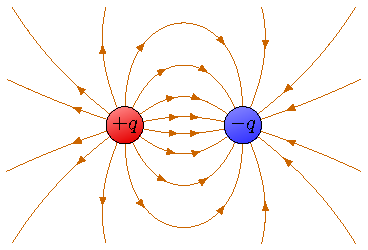
\includegraphics[page=1, width=0.4\textwidth]{pictures/dipole.pdf}}%
    \hspace*{0.2\textwidth}%
    \subfloat[Far field]{\includegraphics[page=2, height=0.3\textheight]{pictures/dipole.pdf}}

    \caption{Dipole in near- and far-field. As we see, the far-field case has a much simpler structure compared to the near-field case, where field lines come in many different forms and shapes. Adapted from \url{https://tikz.net/electric_fieldlines2/}.}
    \label{fig:dipoles}
\end{figure}



            \paragraph{Quadrupole}
now we put two dipoles together in opposite orientation, to eliminate dipole moment. next leading order is thus a quadrupole



        \subsection{Conductors}
Until now, all theory we treated happened in vacuum, i.e.~no charges were present outside the ones described by $\rho$. Next, we turn our attention to electric fields in matter. We can divide matter into three different categories, when it comes to their properties regarding charges and interactions with electric fields: \Def[insulator]{insulators} with no free charges, \Def[conductor]{conductors} with one or more free electrons per atom, and \Def[dielectricum]{dielectrics} which are somewhere in between. Insulators do not react in any significant way to external electric field, so discussing them here is kind of pointless. Dielectrics are interesting and we dedicate the next subsection to them. This one is focussing on conductors.


As we already said, conductors have free charges inside of them, i.e.~electrons attached to atoms that are basically free to roam around in the material. If the number of free charges was infinity, we would call the material a \Def{perfect conductor}. While this is of course not possible in reality, many materials (especially metals) come very close to that and such an approximation is justified. (This is not so different from using a continuous charge distribution $\rho$. In reality, there is always a finite number of particles occupying discrete positions in space, but using $\rho$ can still be more convenient and thus justified.)

Let us now note down some properties, which immediately follow from this definition.

definition: has unlimited amount of free charges


-> fields are cancelled because there are so many free charges


Nice thought experiment: what happens if we have a hole (cavity) inside of a conductor? Does it contain a field? Does the answer to this depend on whether the cavity itself contains charge?

-> field in space that contains no charges, but is surrounded by a conductor, must be zero -- if there were any field lines, where would the begin and end? Would have to be on the conducting surface, but there \todo{finish argument}; this construction is called a \Def{Faraday cage}



        % \subsection{Isolators}
        % \subsection{Dielectrica}
        \subsection{Dielectric Media}
\todo{make whole section? \enquote{Electrostatics Of Dielectrica}?}



idea of what changes in a medium: total electric field now comes from free charges in $\rho$ \emph{and} from charges in the medium; we assume no free charges in medium for now, but still a total charge can be induced via the formation of small dipoles in the medium -> we look at the macroscopic effect only, i.e.~polarization $\vec{\mathbb{P}}$\footnote{We do not call it $\vec{P}$ here because this is already reserved for momentum.}

-> sign of polarization (in Maxwell equation; i.e.~that we add to total electric field in order to get field from free charges, instead of subtracting) comes from sign we choose for dipole moment, right? Or sign of field lines or something, which then affects in which direction dipoles are formed, something like that

-> Maxwell with divergence then only valid for field coming from free charges (not in medium due to all the constraints we have there, as very hand-wavy explanation)



        \subsection{Boundary Conditions}
\todo{look at Griffiths 2.3.5}
We have seen that boundary conditions play an important part in obtaining the electric field (and thereby interaction between charges) during our discussions of the Poisson equation. Normally, boundary conditions are specified as part of the problem, i.e.~they are given to us by the physical setup. But they cannot be arbitrary, as we can see by thinking in general about the behavior of static electric fields at a boundary surface with surface charge $\sigma$. Our tool to study this has, not surprisingly, been developed by Gauss and is called a \Def{Gaussian pillow} (Fig.~\ref{fig:gaussian_pillow}).



\begin{figure}
    \centering

    \subfloat{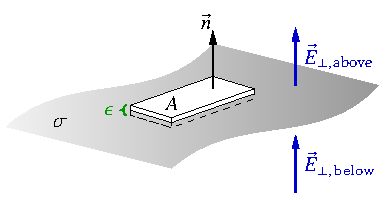
\includegraphics[width=0.45\textwidth,page=1]{pictures/gauss_pillow.pdf}}%
    \hspace*{0.1\textwidth}%
    \subfloat{\includegraphics[width=0.45\textwidth,page=2]{pictures/gauss_pillow.pdf}}

    \caption{Heavily inspired by Figs.~2.36, 2.37 in \cite{Griffiths_2017}. Note that $\vec{E}_{\perp, \parallel}$ are meant to be the fields in the immediate (in fact, infinitesimal) vicinity of the surface.}
    \label{fig:gaussian_pillow}
\end{figure}



            \paragraph{In Free Space}
Let us begin by discussing the case where no medium present outside of the boundary surface. 


-> we enclose very small volume $\mathcal{V} = A \epsilon$, in fact we are interested in $\epsilon \rightarrow 0$ (and, depending on the shape of the surface and how quickly the field $\vec{E}$ varies with position, we might also have to look at $A \rightarrow 0$)

-> idea: evaluate same expression twice, once explicitly and once using Gauss's law

-> second one yields $\int_{\mathcal{S} = \partial \mathcal{V}} \vec{E} \cdot d\vec{\mathcal{S}} = \frac{Q(\mathcal{V})}{\epsilon_0} = \frac{A \sigma}{\epsilon_0}$

-> for explicit evaluation let's look at contributions more closely (we can divide surface and add up integrals): top and bottom each give contribution of the kind $\int_A \vec{E} \cdot d\vec{A} = E_\perp A$ where $E_\perp$ is the field above and below the surface, respectively (which is parallel to the normal vector of $A$ and, if we choose $A$ sufficiently small, constant over it, this is how result comes to be); but when we evaluate the expression for every other area is proportional to $\epsilon$, so the contribution vanishes; accounting properly for orientations of the surfaces (given by their normal vectors), we are left with
\begin{equation}\label{eq:bound_cond_estat_vacuum_1}
    \eqbox{
        E_{\perp, \mathrm{above}} - E_{\perp, \mathrm{below}} = \frac{\sigma}{\epsilon_0}
    } \, .
\end{equation}
(which is also valid in the limit $A \rightarrow 0$ because the $A$'s on both sides cancel.) The electric field is discontinuous when it goes through a surface that has surface charge $\sigma \neq 0$. The latter is the most important part here, though, in case of a uniformly charged sphere for instance the field is actually continuous.


-> selecting any of the surfaces on side of the pillow, we can also calculate the line integral along their boundary $\mathcal{C}$ (e.g., the red line in Fig.~\ref{fig:gaussian_pillow}):
\begin{equation*}
    \int_{\mathcal{C} = \partial \mathcal{S}} \vec{E} \cdot d\vec{r} = E_{\parallel, \text{above}} l - E_{\parallel, \text{below}} l - E_{\perp, \text{above}, \text{left}} \frac{\epsilon}{2} - E_{\perp, \text{below}, \text{left}} \frac{\epsilon}{2} + E_{\perp, \text{above}, \text{right}} \frac{\epsilon}{2} + E_{\perp, \text{below}, \text{right}} \frac{\epsilon}{2}
\end{equation*}
where $l$ is the length of one of the edges of the pillow (the one indicated in Fig.~\ref{fig:gaussian_pillow}). In the limit $\epsilon \rightarrow 0$, many terms do not survive. Further, we must recognize that the integral along a boundary $\partial \mathcal{S}$ is a closed integral by definition -- but then it must be zero, according to the second Maxwell equation (cf.~Eq.~\eqref{eq:maxwell_estat_two}). Therefore, the tangential components fulfil
\begin{equation}\label{eq:bound_cond_estat_vacuum_2}
    \eqbox{
        E_{\parallel, \text{above}} = E_{\parallel, \text{below}}
    }
\end{equation}

Using $\vec{E} = \vec{E}_\perp + \vec{E}_\parallel$ the two conditions on $\vec{E}$ can be summarized in a single, concise equation:
\begin{equation}\label{eq:bound_cond_estat_vacuum}
    \eqbox{
        \vec{E}_\text{above} - \vec{E}_\text{below} = \frac{\sigma}{\epsilon_0} \vec{n}
    } \, .
\end{equation}



In terms of potential, these equations read
\begin{equation}
    \grad \varphi_\text{above} - \grad \varphi_\text{below} = - \frac{\sigma}{\epsilon_0} \vec{n}
\end{equation}
(reminder: $\vec{n}$ is the unit normal vector to the surface) or, defining the \Def{normal derivative}
\begin{equation}
    \eqbox{
        \pdv{\varphi}{n} \coloneqq \vec{n} \cdot \grad \varphi
    } \, ,
\end{equation}
they take the form
\begin{equation}
    \eqbox{
        \pdv{\varphi_\text{above}}{n} - \pdv{\varphi_\text{below}}{n} = - \frac{\sigma}{\epsilon_0}
    } \, .
\end{equation}


But while the gradient of the potential inherits a discontinuity from the field, the potential itself \emph{is} continuous since
\begin{equation}
    \varphi_\text{above} - \varphi_\text{below} = \int_{-\epsilon/2}^{\epsilon/2} \vec{E} \cdot d\vec{r} \underset{\epsilon \rightarrow}{=} 0
    \quad \Leftrightarrow \quad
    \eqbox{
        \varphi_\text{above} = \varphi_\text{below}
    } \, .
\end{equation}
(We omit integration over the other spatial dimensions here since only the one in the direction normal to the surface matters.)



            \paragraph{In A Medium}
?or should we say in a dielectric?



    \section{Magnetostatics}
Even if no electrical field is generated by a conductor, it is possible to have moving charges, i.e.~a \Def{current} (has a direction, parallel to electric field lines, i.e.~from $+$ to $-$). The strength of the current $I$ (often simply called \Def{current}) is usually quantified as the amount of charge flowing through a certain area in a given time. At a given point, $dq$ over the time interval $dt$ depends on the charge density $\rho$ at this point in space (and time), the velocity $v$ with which the charges move, and the area element $d\mathcal{S}$ the flow of charges is analyzed for. All in all,
\begin{equation}
    % \eqbox{
        dq = \rho \, v \, dt \, d\mathcal{S}
    % }
    \quad\Rightarrow\quad
    \eqbox{
        I \coloneqq \dv{q}{t} = \rho v d\mathcal{S}
    } \, .  
\end{equation}
Based on the current, it is common to define a \Def{current density} $j$ that quantifies the flow per area element $d\mathcal{S}$. Since the flow of charges we are talking about naturally is a quantity with a direction, it makes sense to define it as a vectorial quantity. More specifically, it makes sense to choose as its direction the normal vector $\vec{n}_\mathcal{S}$ of the area $d\mathcal{S}$, since this is the direction of charge flow (i.e.~also the direction of $\vec{v}$). Hence,
\begin{equation}
    \eqbox{
        \vec{j}(\vec{r}, t) \coloneqq \dv{I}{\mathcal{S}} \vec{n}_\mathcal{S} = \rho(\vec{r}, t) \, \vec{v}(\vec{r}, t)
    } \, .
\end{equation}
Note that this is a general definition, we are still in magneto\emph{statics}, so $\rho, \vec{v}$ are independent of $t$ for now.
% Further note that for currents that are uniform over the whole $\mathcal{S}$ of interest, division by the area element amounts to division by $\mathcal{S}$. -> this is just wrong. In integration, this becomes important
\\


Now suppose that we observe a change in the total charge in some volume, $Q(\mathcal{V})$. In the absence of loss processes like heat loss, such a change in charge must be complemented by some current flowing out of the volume's boundary $\mathcal{S} = \partial \mathcal{V}$. Mathematically, in integral form
\begin{equation}\label{eq:cont_eq_int}
    \eqbox{
        % \pdv{Q}{t} = \pdv{t} \int_\mathcal{V} \rho \, d\mathcal{V} = \int_\mathcal{S} \pdv{\rho}{t} d\mathcal{S}
        \pdv{Q}{t} + \int_\mathcal{S} j \, d\mathcal{S} \todo{$\vec{j} \cdot d\vec{\mathcal{S}}$?} = 0
    }
\end{equation}
For the 2D-generalization of a test charge (sometimes called \Def{filamentary current}), i.e.~something like a cable of infinitesimal diameter (so that charges can only enter at start and end of it), this takes the form $\dv{Q}{t} = I_A - I_B$ ($A$ is the label for the start of the cable, $B$ for the end). Note that the sign here is a consequence of how we defined current, namely parallel to the field lines. Consider a positive charge moving along the current from $A$ to $B$ and leaving the volume $\mathcal{V}$. Then it leaves in $B$, meaning the current $I_B$ is larger than $I_A$, so that the right hand side of the continuity equation becomes negative. This corresponds to the $Q(\mathcal{V})$ decreasing, which is what we expect since a positive charge is leaving $\mathcal{V}$.


Using that $\pdv{t}$ and $\int_\mathcal{V} d\mathcal{V}$ may be interchanged, and applying Gauss's law we obtain the differential form of Eq.~\eqref{eq:cont_eq_int}
\begin{equation}\label{eq:cont_eq_diff}
    \eqbox{
        \pdv{\rho}{t} + \div \vec{j} = 0
    } \, .
\end{equation}
This is the (differential form of the) \Def{continuity equation}, which just expresses in mathematical terms conservation of charge. (Note that we operate under the assumption that no charges are created in $\mathcal{V}$, otherwise there would be an extra term on the right hand side of the equation.) Its validity can be proven from the Maxwell equations.


\todo{treat Ohm's law! In form $\vec{j} = \sigma_\mathrm{el} \vec{E}$}



        \subsection{Magnetic Force}
For the net electric field coming from a volume $\mathcal{V}$, it does not matter whether the charges generating the field are moving or not; if the total charge $Q(\mathcal{V}) = 0$, then $\mathcal{V}$ produces no field, so no force is felt by two particles with opposite charge sitting next to it.\footnote{We take two particles here to produce a situation with no net charge. The whole point of this example is that a force is acting without any net charge being present.} But here is something curious: suppose the two particles now starts moving. Then, what we observe in an experiment is that they suddenly experience a force. How can this be explained?


From a modern day perspective, the proper approach is to perform a relativistic analysis of the situation, which indeed yields the correct results and laws. The reason why two moving charges still feel a force is, in two words, length contraction. In the rest frame of $\mathcal{V}$, particles moving away it see the charge density $\rho$ constituting the current to be contracted, so that these moving particles a net electric field that exerts a Coulomb force $q \vec{E}$. (Yes, this effect even occurs for non-relativistic speeds, despite the length contraction being incredibly small. This is because the electric force is very strong.)


The problem is that relativity theory did not exist when the aforementioned effect was discovered around $\sim$1800, so another explanation was brought forward. The natural conclusion from the observations was that another force is acting, caused by another field -- this is how the \Def{magnetic field} was born. Biot and Savart \todo{really? why is it Lorentz force then?} empirically found the force exerted from current $\vec{j}_1$ onto current $\vec{j}_2$ to be
\begin{equation}
    \eqbox{
        \vec{F}
        = \fpmu \int_{\mathcal{V}'} \\mathcal{V} \vec{j}_2(\vec{r}') \cross \qty[\vec{j}_1(\vec{r}) \cross \frac{\vec{r}' - \vec{r}}{\norm{\vec{r}' - \vec{r}}^3}] \, d\mathcal{V} \, d\mathcal{V}'
        % \eqqcolon \int_{\mathcal{V}'} \vec{j}_2(\vec{r}') \cross \vec{B}_1(\vec{r}') \, d\mathcal{V}'
    }
\end{equation}
This is the \Def{Lorentz force}, in the special case of vanishing electric field. (The full Lorentz force can be obtained by adding the Coulomb force $\vec{F} = q \vec{E}$ to the expression above.) The magnetic field \todo{B is flow?flux? density} (also: \Def{magnetic induction}), denoted by $\vec{B}$, now comes in by rewriting this in a very particular form, namely as
\begin{equation}\label{eq:biot_savart_general}
    \eqbox{
        \vec{F}
        \eqqcolon \int_{\mathcal{V}'} \vec{j}_2(\vec{r}') \cross \vec{B}_1(\vec{r}') \, d\mathcal{V}'
    }
    , \quad
    \eqbox{
        \vec{B}_1(\vec{r}') = \fpmu \int_\mathcal{V} \vec{j}_1(\vec{r}) \cross \frac{\vec{r}' - \vec{r}}{\norm{\vec{r}' - \vec{r}}^3} \, d\mathcal{V}
    }
\end{equation}
The second equation is called \Def{Biot-Savart law}\footnote{Actually, Biot and Savart found a special case of this general law, where both currents are filamentary currents, whence the volume integrals reduce to line integrals. The same goes for the term \enquote{Ampere force}.}, while the first one is called \Def{Ampere force}.

-> $B$ has units of Tesla, $1 \mathrm{T} = 1 \frac{\mathrm{N}}{\mathrm{A} \mathrm{m}}$

-> $\mu_0$ is magnetic field constant

-> $B$ is not field strength, but flow density \todo{find proper term(s) -> flux?}; $E$ is field strength, $D$ is flow density; later we will see field strength $H$


\begin{ex}[Magnetic Field of a Filamentary Current]
    for filamentary current, the wall thickness/are $dS \rightarrow 0$, which means $j \rightarrow \infty$. However, $\int_\mathcal{V} \vec{j} d\mathcal{V} = \int_\mathcal{V} j \vec{n}_\mathcal{S} \, d\mathcal{S} \, dr = \int_\mathcal{C} \int_\mathcal{S} \dv{I}{\mathcal{S}} d\mathcal{S} \, \vec{n}_\mathcal{S} dr = \int_\mathcal{C} I d\vec{r}$ where $\mathcal{C}$ is the curve following the filamentary current and $d\vec{r}$ is the line element of $\mathcal{C}$. $I$ denotes the current at each point in the filament.

    this is original Biot-Savart law; corresponding force is called Ampere force
\end{ex}

-> we can do something very similar to Gauss law, rearrange this and see: there is (a) potential!



        \subsection{Maxwell Equations}
Brute-force calculation shows that we can rearrange
\begin{equation}
    \eqbox{
        \vec{B}(\vec{r}) = \curl \vec{A}(\vec{r})
    }
    \, , \quad
    \eqbox{
        \vec{A}(\vec{r}) = \fpmu \int_{\mathcal{V}'} \frac{\vec{j}(\vec{r}')}{\norm{\vec{r} - \vec{r}'}} \, d\mathcal{V}'
    } \, .
\end{equation}
with a \Def{vector potential} $\vec{A}$. A direct implication is that $\vec{B}$ is divergence-free, i.e.
\begin{equation}\label{eq:maxwell_magnstat_one_diff}
    \eqbox{
        \div \vec{B} = 0
    } \, .
\end{equation}
This is the first Maxwell equation of magnetostatics.

-> tells us that there are no magnetic monopoles! Crucial difference to electric fields. (In fact, one can write each vector field as the sum of a divergence-free and a curl-free part, $\vec{E}$ and $\vec{B}$ behave kind of opposite to each other.)

The second one follows from a mathematical theorem, which states that the divergence-free part of a vector field (and thus in case of $\vec{B}$ the whole field) may be calculated:
\begin{equation*}
    \vec{B}(\vec{r}) = \curl \frac{1}{4 \pi} \int_{\mathcal{V}'} \frac{\curl \vec{B}(\vec{r}')}{\norm{\vec{r} - \vec{r}'}} \, d\mathcal{V}'
    \, .
\end{equation*}
Comparing this with Eq.~\eqref{eq:biot_savart_general} immediately yields the second Maxwell equation of magnetostatics,
\begin{equation}\label{eq:maxwell_magnstat_two_diff}
    \eqbox{
        \curl \vec{B} = \mu_0 \vec{j}
    } \, .
\end{equation}
In integral form, the two equations read
\begin{equation}\label{eq:maxwell_magnstat_one_int}
    \eqbox{
        \oint_{\partial \mathcal{V}} \vec{B} \cdot d\vec{\mathcal{S}} = 0
    }
\end{equation}
and
\begin{equation}\label{eq:maxwell_magnstat_two_int}
    \eqbox{
        \oint_{\mathcal{C}} \vec{B} \cdot d\vec{r} = \mu_0 I
    }
\end{equation}
\todo{clarify on this. is curve really closed? what is $I$ here, the total current through the curve or something?}

-> first one tells us total flux of $\vec{B}$ through the surface of a volume is zero; second one is Ampere's law, which tells us about sources of magnetic field


We can further express Eq.~\eqref{eq:maxwell_magnstat_two_diff} in terms of the vector potential $\vec{A}$:
\begin{equation}
    \mu_0 \vec{j} = \curl \vec{B} = \curl \qty(\curl \vec{A}) = \div \qty(\div \vec{A}) - \laplacian \vec{A}
    \, .
\end{equation}

-> now we come to interesting part, namely gauge freedom of the theory; by working in Coulomb gauge, we can turn this into wave equation



    \section{Electrodynamics}
In statics, the electric field is curl-free and the magnetic field is divergence-free. As we will see, this changes when looking at electrodynamics, and not just that, there will be a mixing and interaction of electric, magnetic field. More detailed analyses of the interplay between the two fields, and especially a relativistic treatment, then reveals that the two are manifestations of one and the same phenomenon, an electromagnetic field. The electric (magnetic) field only arise in the special cases of electro(magneto-)statics as the curl-(divergence-)free components of this electromagnetic field.


We can already see that the lines between electric and magnetic fields are actually more blurry than they seem by studying a very simple example, the interaction of two moving point charges. (Note that this is neither a problem from electrostatics nor from magnetostatics, since there are both net charges and currents in this setup. Thus it falls into the realm of electrodynamics).

% -> basically: is due to length contraction, moving charge sees different distribution of charges than resting. Historical approach: introduce new field and force, magnetic field. This complements electrical interaction between two charges, both of which are moving.

% -> better wording: can be analyzed/explained entirely by a proper relativist analysis of the situation. Results match what was found empirically be Biot and Savart


% From a modern perspective, with relativity theory developed (this was not the case when these effects were found), it would be straightforward to look at electric field in rest frame of charges moving in the current and then transform back into an \enquote{external}, inertial frame. Historically speaking, however, relativity theory was not there when the aforementioned effect was discovered. Therefore, it was the most natural thing to associate it with new physics, and this is how the \Def{magnetic field} came into existence.
% \footnote{For a very clear, yet concise derivation of the laws of electromagnetism from Coulomb's law (i.e.~electrostatics), see this article by Leigh Page: \url{https://zenodo.org/record/1450178}.}



\begin{ex}[Two Moving Point Charges]\label{ex:point_charge_magn_field}
    Verbally/In words, I can claim a lot, for instance that electric and magnetic field are essentially the same thing viewed from different frames, but do these claims hold up when looking at actual expressions? For that, let us look at the simples scenario possible, the force between two currents made up of a single test charge each, i.e.~$\vec{j}_i = q_i \vec{v}_i \, \delta (\vec{r} - \vec{r}_i)$. In that case, the Biot-Savart law reads
    \begin{equation}
        \vec{B}_1(\vec{r}) = \fpmu q_1 \vec{v}_1 \cross \frac{\vec{r} - \vec{r}_1}{\norm{\vec{r} - \vec{r}_1}^3}
    \end{equation}
    and the corresponding Lorentz force exerted on the second particle becomes
    \begin{align}
        \vec{F} &= q_2 \vec{v}_2 \cross \vec{B}(\vec{r}_2) = \fpmu \frac{q_1 q_2}{\norm{\vec{r}_2 - \vec{r}_1}^3} \vec{v}_2 \cross \qty[\vec{v}_1 \cross (\vec{r}_2 - \vec{r}_1)]
        \notag\\
        &= \fpmu \frac{q_1 q_2}{\norm{\vec{r}_2 - \vec{r}_1}^3} \qty[(\vec{v}_2 \cdot (\vec{r}_2 - \vec{x_1})) \vec{v}_1 - (\vec{v}_2 \cdot \vec{v}_1) (\vec{r}_2 - \vec{r}_1)]
        \notag
    \end{align}
    If you are trained in relativity, then you will recognize that does look a lot like a Lorentz transform (even more so since $\mu_0 = \frac{1}{c^2 \epsilon_0}$). To see this in even more detail, let us assume that $\vec{v}_1 \parallel \vec{v}_2 \parallel \vec{e}_x$ while the displacement vector is $\vec{r}_2 - \vec{r}_1 \parallel \vec{e}_y$. In that case,
    \begin{align}
        \vec{F} &= \fpmu \frac{q_1 q_2}{\norm{\vec{r}_2 - \vec{r}_1}^3} \qty[(\vec{v}_2 \cdot (\vec{r}_2 - \vec{x_1})) \vec{v}_1 - (\vec{v}_2 \cdot \vec{v}_1) (\vec{r}_2 - \vec{r}_1)]
        \notag\\
        &= - \frac{v_1 v_2}{c^2} \fpeps q_1 q_2 \frac{\vec{r}_2 - \vec{r}_1}{\norm{\vec{r}_2 - \vec{r}_1}^3}
        \notag
    \end{align}
    However, this is not the total Lorentz force yet. Since there is only one test particle for each current in this setup, the electric field is not vanishing. Therefore, the Coulomb force between the particles is also acting and due to the superposition principle for forces, we can simply add the term $q \vec{E}_1(\vec{r}_2)$ to $\vec{F}$, which yields the total Lorentz force
    \begin{equation}
        \vec{F} = \fpeps q_1 q_2 \frac{\vec{r}_2 - \vec{r}_1}{\norm{\vec{r}_2 - \vec{r}_1}^3} - \frac{v_1 v_2}{c^2} \fpeps q_1 q_2 \frac{\vec{r}_2 - \vec{r}_1}{\norm{\vec{r}_2 - \vec{r}_1}^3} = \fpeps q_1 q_2 \frac{\vec{r}_2 - \vec{r}_1}{\norm{\vec{r}_2 - \vec{r}_1}^3} \qty(1 - \frac{v_1 v_2}{c^2})
        \notag\, .
    \end{equation}
    where we have further simplified the setup by choosing the test charges to be exactly co-moving, $v_1 = v_2$.\footnote{Granted, this step is mostly done to arrive quickly at a convenient expression, but in my understanding, this simply avoids doing two Lorentz transforms because for $v_1 = v_2$, the rest frame of both test charges is the same. A justification of this is given by the existence of general treatments, which we mention later on.} This equation can be further rewritten by making use of the Lorentz factor $\gamma = (1 - v^2 / c^2)^{-1/2}$:
    \begin{equation}
        \eqbox{
            \vec{F} = \fpeps q_1 q_2 \frac{\gamma(\vec{r}_2 - \vec{r}_1)}{\gamma^3 \norm{\vec{r}_2 - \vec{r}_1}^3}
        }
        \, .
    \end{equation}
    -> some more stuff goes into this (perhaps already in equation before); we assume that difference only has non-zero components in direction that particles move (otherwise gamma in front of vector difference does not work); is fine, but must be mentioned -> actually this might not even be the case

    -> mention that even in non-relativistic case we get correct result -> ah, but then we have electric field mostly... This is difference to Feynman lecture example, where no net charge, so that B-field is \emph{only} field left (then the argument of \enquote{electric interaction so strong that this tiny length contraction has effect even for non-relativistic speeds} makes sense, here not so much)

    Therefore, we see that the Lorentz force exerted in a frame relative to which the point charges move is essentially a boosted version of the Lorentz force in a frame where the charges are stationary. Length contraction changes how the field is perceived in this frame. Granted, we have made many simplifying assumptions here (and also look only at the three-vector $\vec{F}$ here), but sources like \cite{Rosser_1968}, Chapter 3., or \cite{Page_1912} show how this can work in very general setups. Our treatment is merely meant to be an outline of the general strategy used to show the acclaimed equivalence.

    \todo{is this really what we intend to show?} -> yes, it is; from inertial frame with respect to which the charges are moving, it looks like the two charges are interacting via Coulomb force over distance $\norm{\vec{r}_2 - \vec{r}_1}$, and the associated currents are interacting via magnetic force over the same distance; however, what we see upon rewriting is that the total Lorentz force is just a Coulomb force, but acting over a contracted distance $\norm{\vec{r}_2 - \vec{r}_1}$ (analyzing from the rest frame, this is the value that the moving charges measure for their separation)

    \todo{draw simply TikZ plot of situation?}
\end{ex}
To summarize this example, relativity shows in quite natural (and, arguably, quite elegant) manner that electric and magnetic force are manifestations of the same phenomenon. It unifies the treatment of problems involving charges and explains different contributions, e.g., to the Lorentz force. So, why does the majority of textbooks still take the approach to explain them separately? Well, in the end still kind of independent because we can treat as separate effects (though mixing is frame-dependent)

-> still makes sense to treat separately, what we have here is really mainly due to movement (as initial thought experiment shows), so the two manifestations occur in independent setups (though, of course, one can have both at a time; this is realm of electrodynamics)





%         \subsection{Faraday's Law}
% Not only do we allow for both electric and magnetic fields now, we also allow these fields to vary with time.


% treat electromotive force



        \subsection{Maxwell Equations}
Now that we impose no restrictions on the configuration of charges, we have to study a few more interactions in addition to those that have been treated already. Our expectation is that electric and magnetic field are gonna mix, as we have already seen in example \ref{ex:point_charge_magn_field} with point charges, simply because we can now have non-vanishing charge and motion of said charge at the same time.

Interestingly, in order to do time-independent electrodynamics, i.e.~electromagnetism, the only thing we have to do is take the Maxwell equations from electro-, magnetostatics and continue with this set of equations. It is only when we go to dynamics with $\pdv{\vec{E}}{t} \neq 0$ and/or $\pdv{\vec{B}}{t} \neq 0$ that we have to do more work. This should be intuitive because any change in the two fields can potentially cause charges to move around, due to the changing force that acts on them. This in turn would influence the fields themselves.\\


Faraday analyzed experimentally the effects of a time-dependent magnetic field and was able to derive the following relationship:
\begin{equation}\label{eq:maxwell_edyn_one_int}
    \eqbox{
        \oint_\mathcal{C} \vec{E} \cdot d\vec{r} = - \int_{\mathcal{S}(\mathcal{C})} \pdv{\vec{B}}{t} \cdot d\vec{\mathcal{S}}
    }
\end{equation}
where $\mathcal{S}(\mathcal{C})$ is the area that is enclosed by $\mathcal{C}$ (equivalently, we could replace $\mathcal{C} \mapsto \partial \mathcal{S}, \mathcal{S}(\mathcal{C}) \mapsto \mathcal{S}$). This is the (integral form of the) first Maxwell equation of electrodynamics. To honor its discoverer, this equation is also called \Def{Faraday's law}. In differential form, it reads
\begin{equation}\label{eq:maxwell_edyn_one_diff}
    \eqbox{
        \curl \vec{E} = - \pdv{t} \vec{B}
    } \, .
\end{equation}
In other words, the only situation where an electric field can have broken symmetry in the form of vortices is when a time-varying magnetic field is present. This symmetry breaking manifests as non-zero line integrals over a closed path.


A time-dependent electric field (here quantified by the field $\vec{D}$ that the free charges emit) must be accompanied by a change in the associated charge density $\pdv{\rho}{t}$, which implies there must be charges moving around, i.e.~a new current. Through some considerations involving the continuity equation, one arrives at the conclusion that the corresponding current density is nothing but $\pdv{t} \vec{D}$. Adding this to the currents that appear in the Maxwell equation in statics then yields the second Maxwell equation of electrodynamics,
\begin{equation}\label{eq:maxwell_edyn_two_diff}
    \eqbox{
        \curl \vec{H} = \vec{j} + \pdv{\vec{D}}{t}
    } \, .
\end{equation}
The corresponding integral form is \todo{verify this equation}
\begin{equation}\label{eq:maxwell_edyn_two_int}
    \eqbox{
        \oint_\mathcal{C} \vec{H} \cdot d\vec{r} = I + \oint_{\mathcal{S}(\mathcal{C})} \pdv{\vec{D}}{t} \cdot d\vec{\mathcal{S}} = I - \epsilon_0 \pdv[2]{t} \vec{B} + \oint_{\mathcal{S}(\mathcal{C})} \pdv{\vec{\mathbb{P}}}{t} \cdot d\vec{\mathcal{S}}
    }
\end{equation}
where $\mathcal{S}(\mathcal{C})$ is the area that is enclosed by $\mathcal{C}$.


\todo{treat electromotive force}

-> some high leven overview: basically, Maxwell equations determine curl and divergence of the two fields $\vec{E}, \vec{B}$, thereby determining the whole field (by mathematical theorem). The corresponding four equations can be divided into homogenous (only the fields interplay) and inhomogeneous (charge and current density appear) ones. Moreover, if we have some medium involved, there are material equations (so some statements from above must be rephrased in terms of other variables; does not really change interpretation, though).

-> these Maxwell equations are complemented by the Lorentz force, total expression of which we sneaked into example \ref{ex:point_charge_magn_field} already, and which reads
\begin{equation}
    \eqbox{
        \vec{F} = q \qty(\vec{E} + \vec{v} \cross \vec{B})
    } \, ,
\end{equation}
where $q, \vec{v}$ represent the charge, velocity of the particle in consideration.


-> more common approach than solving Maxwell equations (kind of annoying, complicated): solve equivalent equations for potentials (so that Maxwell are automatically fulfilled), determine fields from potentials; in statics, this amounted to solving Poisson equations, and here ...

for potentials in Lorenz gauge, generalization of Poisson reads
\begin{equation}
    \eqbox{
        \square \varphi = - \frac{\rho}{\epsilon_0}
    }
    \manyqquad
    \eqbox{
        \square \vec{A} = - \mu_0 \vec{j}
    } \, .
\end{equation}



    \section{Notes}

so we can we take viewpoint that there are truly only two Maxwell equations, for field tensor? And one of them being ($dF = 0$) that electromagnetic force is conservative (which directly implies we can find potential)



\end{document}